%Tu si môžete zaznačiť, že pracujete na danej veci. V prípade, že ste napísali len časť a ďalej už
%nechcete, alebo ste hotoví tak sa odtiaľ odpíšte. Bolo by však fajn, aby jedu vec robil jeden
%človek ak celok a zvyšný len kontrolovali
%vypracuva: Andrej
\documentclass{article}

\input include/include.tex
\usepackage{hyperref}
\hypersetup{
    colorlinks=true,
    linkcolor=blue,
    filecolor=magenta,      
    urlcolor=blue,
}
\begin{document}

\velkynadpis{Python tutoriál}
\tableofcontents
\newpage

Ahoj, pred oči sa ti dostal Python tutoriál napísaný pri príležitosti Online Školy Programovania 2020. Jeho autormi sú Roman a Andrej (Andrej a Roman), za proofread ďakujeme Žabovi. Ak v tutoriále nájdeš nejaké chyby alebo pasáže, ktoré sme nie zrovna dobre podali, neváhaj nás kontaktovať. Ako môžeš spoznať zle napísanú pasáž? Tak, že ani po niekoľkonásobnom prečítaní nerozumieš tomu, čo text, resp. kód znamená. Kontaktovať nás môžeš buď na Discorde pod nickom sobkulir a Aj0SK alebo na adresách andrejkorman@gmail.com a r.sobkuliak@gmail.com.

\section{Úvod}
Predtým ako s Pythonom začneme, je dôležité zodpovedať niekoľko otázok. Prvá a najdôležitejšia je, čo je programovanie. Programovanie je vytváranie programov, ktoré na počítači vieme spustiť a majú nejakú funkciu. Príkladom programu môže byť aplikácia na četovanie, webový prehliadač ale aj niečo jednoduchšie, ako napríklad kalkulačka. Dôležité na programoch je, že majú vstup a výstup. Pre program fungujúci ako kalkulačka môže byť vstupom matematický výraz typu $5+3\cdot 7$ a výstupom hodnota tohto výrazu $26$. My sa v tomto tutoriále budeme venovať jednoduchým programom. V prípade kalkulačky na vašom počítači ste zrejme zvyknutí zadať matematiký výraz pomocou tlačidiel, teda nejakého grafického rozhrania (tlačidlá, okná a podobne). Takéto rozhranie naše programy nebudú mať, čo ich mimochodom značne skracuje. Vstup aj výstup bude teda v textovej podobe.

Keď už vieme čo je program a chceme programovať, potrebujeme vedieť ako taký program vytvoriť. Na to slúžia, ako už isto tušíte, programovacie jazyky. Tie nám dovoľujú vytvoriť postupnosť príkazov, ktoré po spustení daný program vykoná. Program od nás po spustení dostane nejaký vstup a vyprodukuje naň odpoveď (výstup), ktorú typicky nejako zobrazí, napr. vypíše.

\subsection{Prečo Python?}
Programovacích jazykov existuje neúrekom, my sme vybrali zrovna Python. Prečo? Myslíme si, že jeho príkazy sú prirodzené a zároveň je široko využívaný v praxi. Podľa \href{https://insights.stackoverflow.com/survey/2019#technology-_-programming-scripting-and-markup-languages}{dotazníku StackOverflow z roku 2019} je to druhý najpopulárnejší programovací jazyk. Python vám teda otvorí dvere do mnohých zákutí informatiky :)

\subsection{Inštalácia}
Predtým, než napíšete svoj prvý program, musíte si Python nainštalovať. Existuje rada veľmi pokročilých nástrojov pre programovanie v Pythone. My s nimi zatiaľ pracovať nebudeme, pretože na úvod sú zbytočne komplikované.
Použijeme preto jednoduchý editor s názvom \texttt{Python IDLE}, ktorého autor vytvoril aj samotný jazyk Python. Tento editor podporuje všetky štandardné operačné systémy (Windows, MacOS, Linux) a stiahnuť si ho môžete z \href{https://www.python.org/downloads/}{oficiálnej stránky Pythonu}. Odporúčame nainštalovať si najnovšiu verziu, v čase písania tohto textu je to verzia 3.8.2. Pripravili sme tiež \href{https://www.youtube.com/watch?v=_oLcUfkgxSI}{videonávod k inštalácii}.

\section{Prvé programy a \texttt{print}}
Keď už máme Python nainštalovaný, otvoríme program Python IDLE. To je editor, v ktorom budeme písať naše programy. Zvoľte \texttt{File -> New File} a do nového okna, ktoré sa otvorilo, skopírujte program:
\lstlang{python}\begin{lstlisting}
# Prvy program v Pythone
print(5)
print(5+2+7)
print(7-10)
print(2*15)
print(15/10)
print(15//10)
print(7%3)
\end{lstlisting}
Následne program uložte pomocou \texttt{File -> Save} do ľubovoľného priečinku. Odporúčame vám, aby ste si vytvorili samostatný priečinok, do ktorého budete vaše programy ukladať. Teraz program môžete spustiť pomocou \texttt{Run -> Run Module} alebo stlačením \texttt{F5}. 

Prvý riadok nie je nijak dôležitý ale je potrebné vysvetliť o čo ide. V kóde sa všetko považuje za príkaz a teda by v ňom bolo ťažké zanechať nejakú informáciu pre čitateľa. Na zanechanie komentára, teda nejakého textu pre človeka, ktorý kód číta slúži znak $\#$. Všetko čo napíšeme zaň sa považuje iba za komentár a Python to odignoruje. My vám za týmto znakom budeme zanechávať nejaké odkazy pre vaše lepšie porozumenie naším príkladom. A teraz už poďme na to podstatné.

V tomto programe používame funkciu \texttt{print}. Vieme asi uhádnuť, čo táto funkcia robí -- vypisuje na výstup to, čo je vo vnútri zátvoriek. Napriek tomu by však bolo vhodné vysvetliť, čo je \textit{funkcia}. Ak vám to nebude úplne jasné, nezúfajte, funkcie sú pomerne zložitá vec, ktorej sa bližšie venuje kapitola 10.
Funkcia je nejaká menšia postupnosť príkazov, ktorá sa natoľko opakuje alebo je logicky ucelená, že dostala názov. Vlastne je to taký malý program v programe. Funkcii zväčša dáme niekoľko \textit{parametrov}, teda jej odovzdáme na čom má vykonať operáciu na ktorú je určená.

Vyššie vidíme, že \texttt{print} je funkcia, ktorá má ako parameter to, čo chceme vypísať. Pozrite sa na výstup programu a zamyslite sa, ktoré riadky vás prekvapili. Je logické, že sa výraz $15 / 10$ nevyhodnotil na celé číslo. Špeciálnu pozornosť si zaslúži aj výraz $15 // 10$. Dve delenia v Pythone označujú často používané tzv. celočíselné delenie, teda delenie bezozvyšku. $x // y$ vieme interpretovať ako: "Najviac koľkokrát sa zmestí $y$ do $x$?" Inak povedané ide o klasické delenie s tým, že vynecháme všetko za desatinnou čiarkou.
Zrejme je pre vás novým ešte výraz $7 \% 3$ kde \% označuje zvyšok po delení. Výsledkom tejto operácie je tá časť čísla čo z neho "ostane" po celočíselnom delení. $7\%3=1$ a to preto, že $7//3=2$ a to čo zostalo vieme vyjadriť ako $7 - 2 \cdot 3 = 1$.

V tomto programe sme si v skutočnosti iba ukázali, že \texttt{print} vie vypísať číslo. Všetky výrazy obsahujúce základné matematické operácie sa totiž priamo vyhodnotia na číslo a úlohou \texttt{print} je už len vypísať dané číslo. \texttt{print} vie ale toho samozrejme viac. Skopírujte si do vášho súboru s kódom nasledovný program:

\lstlang{python}\begin{lstlisting}
print("Python tutorial!")
print("Python" + "tutorial!")
print(2 + 3)
print("2" + "3")
\end{lstlisting}

Na prvom riadku vidíme, že vieme vypísať aj text. Takýto text v Pythone nazývame \textit{reťazec znakov} alebo skrátene \textit{reťazec}. Ide o znaky ohraničené úvodzovkami, teda \texttt{\textquotedbl<text>\textquotedbl} alebo \texttt{\textquotesingle<text>\textquotesingle}. Všimnite si, že nezavísi na tom, či použijeme "obyčajné úvodzovky", teda \texttt{\textquotedbl}, alebo apostrof, teda \textquotesingle. Najčastejšie keď hovoríme v Pythone o znakoch, myslíme tým anglickú abecedu, číslice, interpunkciu, zátvorky a podobne. V tomto texte vôbec nepracujeme s dĺžňami, mäkčeňmi a slovenskou abecedou.

V druhom riadku vidíme, že podobne ako čísla, reťazce vieme sčítavať. Čo urobí znamienko plus v tomto prípade je, že zlepí reťazce za seba. Ako je možné, že výsledok 3. a 4. riadku sa líši? Dôvodom je, že v prvom prípade ide o plus aplikované na čísla. V druhom prípade sme aplikovali plus na reťazce. Python vidí, že naľavo aj napravo od plus sa nachádzajú čísla s úvodzovkami okolo čím sme dali najavo, že chceme tieto čísla reprezentovať ako reťazce a Pythonu teda neostáva nič iné, ako použiť plus pre reťazce.
Keď sa pokúsime tieto dve reprezentácie skombinovať a 
napíšeme

\lstlang{python}\begin{lstlisting}
print(2 + "3")
# Chyba! 
# TypeError: unsupported operand type(s) for +: 'int' and 'str'
# Tento program po spusteni skonci chybou vyssie. Python nam v tejto
# chybe hovori, ze operator + nemozno pouzit medzi typmi 'int' a 'str'.
\end{lstlisting}

tak spôsobíme chybu. Je to z dôvodu, že Python nerozumie ako má sčítať \textit{int}, teda \textit{integer} (celé číslo) a \textit{str}, teda \textit{string} (reťazec). Toto neplatí, ak plus nahradíme znamienkom krát. Tak schválne, čo vypíše program:

\lstlang{python}\begin{lstlisting}
print(2 * "Ahoj!")
# Vystup: Ahoj!Ahoj!
\end{lstlisting}

Posledná vec, ktorá sa týka príkazu \texttt{print} je, že po tom, čo tento príkaz vypíše čo sme mu prikázali, ďalšie zavolanie funkcie \texttt{print} v rovnakom programe píše na ďalší riadok. Teraz vám niečo prezradíme. To, že text skočí na ďalší riadok je spôsobené tým, že sa v texte, ktorý vypisujete skrýva znak, ktorý nie je tlačiteľný, teda ho nie je vidieť ale spôsobí, že text za ním je na novom riadku. Tento znak vieme zapísať ako \texttt{\textbackslash n}. Vyskúšať si to môžete tak, že do programu napíšete príkaz:

\lstlang{python}\begin{lstlisting}
print("Tu bude novy riadok->\n a aj tu->\n bol novy riadok.")
# Vystup:
# Tu bude novy riadok->
#  a aj tu->
#  bol novy riadok
\end{lstlisting}

% (fixed) TODO (Žaba): tu mi to príde, že strašne rýchlo a bez vysvetlenia sa pridajú parametre, ešte sa nestretli s tým, že čiarka a pomenované parametre. To by som nevysvetľoval asi do detailov, ale viac by som to spomenul.

Funkcia \texttt{print} tak nerobí nič iné ako to, že pridá na koniec toho, čo chceme vypísať \texttt{\textbackslash n}. Tvorcovia funkcie \texttt{print} na to mysleli a pridali možnosť ako znak nového riadku pri výpise zmeniť. Funkcia \texttt{print} v zátvorkách vždy príjme jednu hodnotu. Túto hodnotu nazývame \textit{parameter}. Parametrov môže mať funkcia viac a oddeľujeme ich čiarkou. Funkcia \texttt{print} má druhý parameter, ktorým vieme ovládať čo bude na konci výpisu. Tento parameter je navyše \textit{pomenovaný}, a asi nás neprekvapí, že sa volá \texttt{end}. Ak by sme teda namiesto znaku nového riadku chceli na konci dve \texttt{X}, spravíme to nasledovne.

\lstlang{python}\begin{lstlisting}
print("Toto cele", end="XX")
print("chcem na jednom riadku.")
# Toto celeXXchcem na jednom riadku.
\end{lstlisting}

Špeciálne, ak za \texttt{print} nechceme vypísať nič, parametru \texttt{end} dáme prázdny reťazec.
\lstlang{python}\begin{lstlisting}
print("Zostavame ", end='')
print("na rovnakom riadku.")
# Zostavame na rovnakom riadku.
\end{lstlisting}

\nadpis{Priklady}

Na konci kapitoly nájdeš vždy sadu úloh, ktoré by si si mal vyriešiť predtým ako budeš pokračovať. Úlohy slúžia na preverenie tvojich schopností a zväčša sa stupňujú v obtiažnosti. V tejto kapitole sme si pre teba prichystali iba jednu úlohu: \href{https://testovac.ksp.sk/tasks/ls-uvod-ahoj/}{Ahoj}

Zrejme si však nikdy ešte neodovzával program na náš testovač a tak ti celý proces v skratke vysvetlíme. Testovač je náš server, kam pošleš svoj program, ktorý rieši nejakú úlohu. Náš testovač tvoj program spustí na rôznych vstupoch a zistí, či robí naozaj to, čo sa v zadaní požaduje. Poďla toho ho ohodnotí OK, WA (wrong answer, nesprávna odpoveď), prípadne nejak inak. Všetky možné výsledky odovzdávania nájdeš v sekcii \texttt{Odpovede testovača}. Neboj sa, o nič nejde a môžeš odovzdávať ľubovoľne veľakrát. Neodporúčame ti ale zaseknúť sa a hodinu riešiť ten istý príklad. Pokiaľ ti príklad nejde a začínaš byť frustrovaný ozvi sa na \href{https://discord.gg/QKgNmW9}{Discorde} v časti začiatočníci alebo napíš priamo jednému z užívaťeľov sobkulir a Aj0SK a my ti radi poradíme.

Teraz už k tomu ako odovzdať svoj program na testovač. Roman pripravil krátky \href{https://www.youtube.com/watch?v=RV5uoLwQDsg}{videotutoriál}. Testovač nájdeš na adrese \href{https://testovac.ksp.sk/}{testovac.ksp.sk}. Prvýkrát zvoľ možnosť \texttt{Zaregistruj sa} a zaregistruj sa ako na hocijakej inej stránke. Po prihlásení sa môžeš stránkou preklikávať pomocou panelu naľavo. Keď sa rozhodneš riešiť, prejdi pomocou panelu naľavo do časti \texttt{Úlohy}

\begin{figure}[h]

\includegraphics[width=4cm]{lavypanel}
\centering
\end{figure}

Potom si všimni sadu príkladov s názvom \texttt{Úvod do programovania} a klikni na \texttt{Zobraziť úlohy} čím sa ti pod týmto tlačidlom vyrolujú úlohy:

\begin{figure}[h]
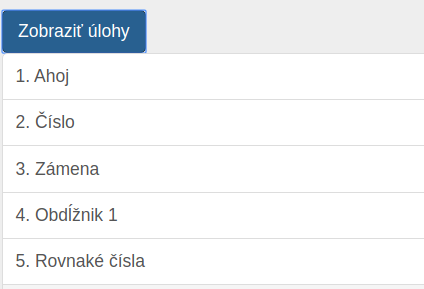
\includegraphics[width=4cm]{zoznam}
\centering
\end{figure}

Po kliknutí na príklad sa už dostaneš na stránku, na ktorú by ťa inak zaviedol link úlohy v tomto tutoriále. Odovzdať príklad môžeš tak, že ho nahráš pomocou tlačidla \texttt{Choose file}, príponu necháš na voľbe \texttt{Zisti podľa prípony} a stlačíš \texttt{Odovzdaj riešenie}. Dôležité je, že po vyriešení úlohy bude toto okno s úlohou vyzerať nejak takto:

\begin{figure}[h]
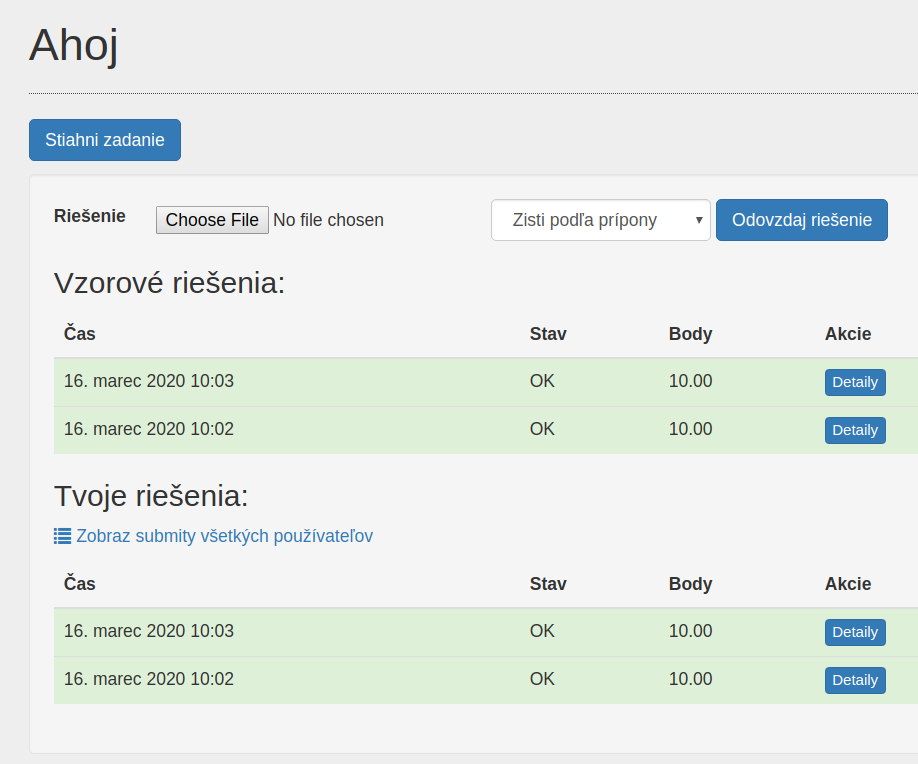
\includegraphics[width=7cm]{vyriesene}
\centering
\end{figure}

Dole sa nachádzajú tvoje submity (pokusy o riešenia), pričom správne riešenie má pri sebe stav OK. Po tom, čo si doriešil úlohu si môžeš rozkliknúť aj \texttt{Vzorové riešenia}, ktoré sú prístupné zväčša v dvoch až troch jazykoch.

\section{Premenné}

Program si k svojmu chodu potrebuje často pamätať nejaké informácie. Či už je to vstup, ktorý programu užívateľ zadal alebo nejaké medzivýsledky výpočtu, ktorý program vykonáva. V Pythone na toto slúžia premenné. Premenná je krabička (miesto v pamäti počítača), kde si program ukladá dáta. Naviac je táto krabička pomenovaná. Akonáhle sa vytvorí krabička s názvom napríklad $x$, vieme do nej uložiť číslo pomocou \texttt{=}.

\lstlang{python}\begin{lstlisting}
x = 4   # do krabicky x vlozime cislo 4
\end{lstlisting}

Neskôr potom vieme použiť hodnotu v tejto krabičke napríklad takto:

\lstlang{python}\begin{lstlisting}
print(4*x)   # pri vyhodnocovani vyrazu sa x nahradi 4
\end{lstlisting}

Do krabičky môžeme hodnotu vložiť a použiť ju aj opakovane.

\lstlang{python}\begin{lstlisting}
a = 10
print(4*x)   # vypise: 40
a = 7
print(4*x)   # vypise: 28
\end{lstlisting}

Zatiaľ sme zatajili ako sa taká premenná vytvára. Tajomstvom je, že python premennú vytvorí automaticky keď jej prvý krát priradíme nejakú hodnotu. Na vytvorenie premennej a priradenie hodnoty do nej teda stačí napísať:

\lstlang{python}\begin{lstlisting}
a = 4   # do a priradime 4, premenna a sa pritom vytvori
b = 2 * a - 3   # do b priradim hodnotu vyrazu napravo, teda 5
c, d = 10, 12   # vieme robit aj viac priradeni naraz (c = 10 a d = 12)
a = 8 # zmenili sme hodnotu a, teraz sa uz premenna znova nevytvorila
\end{lstlisting}

Na začiatku sme hovorili, že do premennej si program ukladá dáta avšak doteraz sme iba ukázali, ako do premennej vložiť číslo. Rôzne typy dát sa nazývajú v programovacích jazykoch aj \texttt{typy}. My sme sa zatiaľ v tomto tutoriále skryto stretli s dvomi typmi. Prvým bolo celé číslo alebo tiež \texttt{int}. Druhým reťazec alebo \texttt{string}. V nasledujúcej tabuľke prinášame aké základné typy v Pythone existujú.

\smallskip
\begin{tabular}{|l|l|l|l|}
\hline
Typ & Slovný popis & Príklady \\ \hline
int & celé čísla & 1, -10, 0, 123 \\ \hline
float & desatinné čísla & 0.5, .3, 3.14  \\ \hline
bool & pravda/nepravda & \texttt{True}/\texttt{False} \\ \hline
string & reťazec znakov & "abc", 'abc' \\ \hline
žiadny & ani jeden z typov & \texttt{None} \\ \hline
\end{tabular}
\smallskip

Ďalším dôležitým pojmom je \texttt{operátor}. Spomenuli sme si už premenné aj to, že majú rôzne typy a vieme ich použiť v akýchsi výrazoch. Pod výrazom myslíme napr. $5\*x + 20 + y$. Tento výraz sa vyhodnotí a vráti sa nám číslo a teda by sme vedeli napísať napr. $vysledok = 5\*x + 20 + y$. V tomto výraze používame operátor $+$ dva krát. $+$ vezme vec napravo, naľavo, sčíta ich a vráti nám výsledok. Python má samozrejme viac operátorov. Niektoré už poznáte ako napr. $-$, $//$, $*$... Vieme už aj o tom, že rovnaký operátor môže fungovať inak keď má napravo a naľavo iné typy a teda vracia aj rôzne typy.

\lstlang{python}\begin{lstlisting}
a, b = 2, 12
c = a+b # c bude 14, + tu vracia cele cislo
r1 = "Ano"
r2 = "Nie"
r3 = r1 + r2 # r3 bude "AnoNie", + vracia retazec
r4 = a * r1 # r4 bude "AnoAno", + vracia retazec
\end{lstlisting}

Aké ešte operátory existujú? Dôležitým typom v programovaní je typ \texttt{bool}. Ten môže reprezentovať iba dve hodnoty a to \texttt{True} a \texttt{False}. Dôležitosť tohto typu sa naplno prejaví v kapitole o podmienkach. Príklad použitia:

\lstlang{python}\begin{lstlisting}
a = True
b = False
print(a)
print(b)
\end{lstlisting}

Operátory, ktorým sme sa doteraz venovali vracali buď celé číslo alebo reťazec. Dôležitými operátormi sú aj tie, ktoré vracajú bool a to $==$ a $!=$. Prvý funguje ako porovnanie, vráti True vtedy keď sa vec napravo a naľavo rovnajú. Druhý je jeho presnou negáciou a teda opakom, vrátu True ak sa vec napravo a naľavo nerovnajú. Príklady použitia:

\lstlang{python}\begin{lstlisting}
a, b = 5, 10
c = (a==b) # v c je False
d = (a==5) # v d je True
e = (a!=b) # v e je True
# pre citatelnost sme vyrazy napravo od = dali do zatvorky
\end{lstlisting}

Ďalšími užitočnými operátoromi, vracajúcimi bool sú $<$, $>$, $>=$ a $<=$. Príklad použitia.

\lstlang{python}\begin{lstlisting}
vysl1 = 5>3 # vysl1 bude True
vysl2 = 7<=8 # vysl2 bude True
\end{lstlisting}

\section{Načítavanie vstupu a výpis výstupu}

% TODO (Žaba): tá vec so zmenou by sa mi dosť páčila príkladovo spraviť. Že vyskúšajme si vyriešiť že máš číslo a vypočítaj obsah štvorca s takou hranou, spravíš reťazec*reťazec, dostaneš chybovú hlášku peknú a na tom vysvetlíš, že aha, toto je zle a takto fixnem.

%TODO (Žaba): chýba načítanie viacerých čísel na riadku (aj konštantne veľa), či to nové úlohy už nebudú mať? Tak či tak, možno spomenúť viac riadkov, to tu tuším nie je. Vidím, že sa to nižšie spomína, ale to už je asi neskoro vzhľadom na príklady?

Na načítavanie používame funkciu \texttt{input}. Po jej použití program načíta jeden riadok zo vstupu
a vráti nám ho ako \textit{reťazec (string)}. My si musíme samozrejme tento reťazec niekam uložiť. Treba si dať pozor na to, že načítaný vstup je reťazec. Ak chceme so vstupom pracovať ako s číslom, musíme ho najskôr \textit{skonverťovať} (premeniť) na číslo pomocou funkcie \texttt{int}.

% TODO (Žaba): tu sú zrazu spomenuté "premenné" ale nikdy predtým sme nevideli ako viac vecí vypísať a asi sa to nedovtípia sami. Buď to niekde doplniť, alebo tu vynechať.

\lstlang{python}\begin{lstlisting}
a = input() # nacita jeden riadok zo vstupu a ulozi ho do premennej a typu string(retazec)
# Chyba! Premenna a obsahuje string, 10 je int.
print(a + 10)

b = int(input()) # ak chceme vytvorit premennu b, typu int, musime retazec skonvertovat na cislo
# Ok, obe premenne su typu int.
print(b + 10)
\end{lstlisting}

Na vypisovanie opäť použijeme funkciu \texttt{print}.
Tej môžeme ako parameter dať napr. premennú/é, ktorú chceme vypísať.

\lstlang{python}\begin{lstlisting}
# Trik: priradenie viacerych premennych naraz. Zapis je ekvivalentny s
# a = 10
# b = 15
a, b = 10, 15
# print s viacerymi parametrami vypise tieto parametre oddelene medzerou
# Pretoze sme nastavili end='', nevypise sa znak konca riadku
print(a, b, end='')
print(a)
# Vystup:
10 1510
# Vysvetlenie:
# Najskor prvy print vypise "10 15" (bez konca riadku)
# a potom druhy print prida 10 (s koncom riadku).
\end{lstlisting}

\nadpis{Priklady}
\href{https://testovac.ksp.sk/tasks/ls-uvod-cislo/}{Číslo},
\href{https://testovac.ksp.sk/tasks/ls-uvod-zamena/}{Zámena},
\href{https://testovac.ksp.sk/tasks/ls-uvod-obdlznik1/}{Obdĺžnik 1}

\section{Podmienky}

Často sa stane, že program potrebuje urobiť nejaké rozhodnutie. Program je vec, ktorá sa správa pri každom spustení rovnako, nie však na každom vstupe. To znamená, že ten istý vstup vždy spôsobí rovnaké správanie programu. Kedže ale programu pri rôznych spusteniach rôzne vstupy je nutné aby na ne program nejako zareagoval. Často napríklad chceme aby sa určitý kód spustil iba za splnenia nejakých podmienok. Príkladom môže byť program, ktorý vypíše, či číslo na vstupe je alebo nie je 0. Vhodným prostriedkom na dosiahnutie tohto správania programu je príkaz \texttt{if}. Ten
zjednodušene vyzerá \texttt{if <podmienka>: <prikaz>}. To znamená, že ak platí \texttt{<podmienka>}
vykonaj \texttt{<príkaz>}. \texttt{<podmienka>} je v tomto prípade akýkoľvek výraz vracajúci \texttt{bool}, teda True alebo False. \textbf{Nezabudnite}, že porovnávanie dvoch vecí sa vykonáva pomocou
\textbf{dvoch} rovná sa \texttt{(==)} a nie jedného\texttt{(=)}.

\lstlang{python}\begin{lstlisting}
x = int(input())
if x == 0:
    print("Je to nula!")
if x != 0:
    print("Nie je to nula!")
\end{lstlisting}

V predchádzajúcom príklade je vidieť ešte jednu dôležitú vec a to odsadenie príkazov. Hovoríme o viditeľnej medzere v 3. a 5. riadku. Odsadením hovoríme pythonu, že tento príkaz patrí k predchádzajúcej podmienke. Je to dôležité z toho dôvodu, keby chceme napr. pri splnení prvej podmienky vykonať viac ako jeden príkaz. V tomto prípade by stačilo len dopísať rovnako odsadený príkaz:

\lstlang{python}\begin{lstlisting}
# Program zisti, ci je na vstupe 0.
x = int(input())
if x == 0:
    print("Je to nula!")
    print("Vypisem este toto!")
    
# Vstup1:
0
# Vystup1:
Je to nula!
Vypisem este toto!

# Vstup2:
3
# Vystup2:
(prazdny)
\end{lstlisting}

Ak by sme druhý výpis neodsadili, \texttt{Vypisem este toto!} by sa vypísalo aj pre nenulový vstup.
\lstlang{python}\begin{lstlisting}
# Program zisti, ci je na vstupe 0.
x = int(input())
if x == 0:
    print("Je to nula!")
print("Vypisem este toto!")
    
# Vstup1:
0
# Vystup1:
Je to nula!
Vypisem este toto!

# Vstup2:
3
# Vystup2:
Vypisem este toto!
\end{lstlisting}

Tak ako v predchádzajúcom príklade sa občas stane, že existujú práve 2 možnosti toho čo chceme urobiť. Vtedy je nápomocný konštrukt \texttt{if <podmienka>: <prikaz> else: <prikaz>}. Teda ak platí podmienka vykonáme prvý príkaz a ak nie tak druhý.

\lstlang{python}\begin{lstlisting}
x = int(input())
if x == 0:
    print("Je to nula!")
else:
    print("Nie je to nula!")
\end{lstlisting}

Poslednou možnosťou je, že máme viac ako 2 možnosti. Vtedy použijeme konštrukt \texttt{if <podmienka>: <prikaz> elif <podmienka>: <prikaz> else: <prikaz>}.
Táto možnosť je vhodná práve keď máme 2 a viac možností pričom chceme aby sa vykonala \textbf{práve jedna}. Počet \texttt{elif} je ľubovolný ale pre čitateľnosť zväčša neodporúčame viac ako $3$-$4$.

\lstlang{python}\begin{lstlisting}
# ak nam nestacia 2 vetvy (if, else), mozeme pridat dalsie pomocou 'elif'
if x % 2 == 0:
  print('x je parne')
elif x % 3 == 0:
  print('x je delitelne 3')
else:
  print('x nie je delitelne ani 2 ani 3')
\end{lstlisting}
Znova si všimnite, že každý príkaz za dvojbodkou je na samostatnom riadku a je odsadený od podmienky.

% TODO (Žaba): neviem či by som namiesto x and y nepoužil formát <podmienka1> and <podmienka2>. Ten sa používal predtým, tu x a y môžu zvládzať k premenným.

Podmienka je ľubovoľný výraz, ktorý vieme vyhodnotiť ako \texttt{True} alebo \texttt{False}.
Takisto však vieme skladať viac výrazov pomocou logických spojok \texttt{and} a \texttt{or}.
Výraz \texttt{x and y} sa vyhodnotí ako \texttt{True} ak sú obe podmienky x, y pravdivé. 
Výraz \texttt{x or y} sa vyhodnotí ako \texttt{True} ak aspoň jedna z podmienok x, y je pravdivá.
V podmienkach môžeme používať zátvorky na zvýšenie prehľadnosti poradia operácii.

\lstlang{python}\begin{lstlisting}
if (x % 2 == 0) and (x % 3 == 0):
  print('x je delitene 6')

# podmienka vyssie je ekvivalentna vnorenym podmienkam
if x % 2 == 0:
  if x % 3 == 0:
    print('x je delitene 6')

if (meno == 'Jozko') or (meno == 'Maria'):
  print('meno je Jozko alebo Maria')
\end{lstlisting}

\nadpis{Priklad}
\href{https://testovac.ksp.sk/tasks/ls-uvod-rovnake/}{Rovnaké},
\href{https://testovac.ksp.sk/tasks/ls-uvod-znamienko/}{Znamienko},
\href{https://testovac.ksp.sk/tasks/ls-uvod-najmensi/}{Najmenší},
\href{https://testovac.ksp.sk/tasks/ls-uvod-prostredny/}{Prostredný},
\href{https://testovac.ksp.sk/tasks/ls-uvod-priemer/}{Priemer},
\href{https://testovac.ksp.sk/tasks/ls-uvod-zvysok/}{Zvyšok},
\href{https://testovac.ksp.sk/tasks/ls-uvod-nenajvacsi/}{Nenajväčší}

\section{Cykly}
V programe potrebujeme často nejakú časť príkazov opakovať viackrát. Napríklad ak by sme potrebovali vypísať čísla od 1 do 5, s doterajšími znalosťami by sme vytvorili nasledovný program.
\lstlang{python}\begin{lstlisting}
print(1)
print(2)
print(3)
print(4)
print(5)
\end{lstlisting}

\subsubsection{While cyklus}
Ako asi už tušíte, musí to ísť aj krajšie. Použijeme preto cyklus \texttt{while} (po slovensky \textit{pokiaľ}).
\lstlang{python}\begin{lstlisting}
# Vypis cisel od 1 do 5.
i = 1
while i <= 5:
  print(i)
  i += 1
\end{lstlisting}

% (fixed) TODO (Žaba): neviem či by som zrovna while ukazoval na príklade, na ktorý je for oveľa lepší. Takisto by sa mi páčila väčšia previazanosť s tou časťou podmienok. Nápad (z brucha, dá sa určite lepší vymyslieť). Chceme zistiť, či je číslo deliteľné 2, super to vieme ifoch. Čo však ak by sme chceli vedieť koľkokrát je deliteľné 2. Tak môžeme spraviť if, potom vydeliť 2 a potom ďalší if...Alebo to môžeme zaobaliť do while. Najlepšie ak by sa dalo skončiť časť s podmienkami pekným príkladom, ktorý potom tu sa rozšíri. Potom sa dá ukázať toto cez while a opäť prejsť k tomu, že for je na to lepší, lebo poznáme počet opakovaní.

Príkaz \texttt{while} opakuje vykonávanie odsadených príkazov, \textit{pokiaľ} platí podmienka uvedená za kľúčovým slovom \texttt{while}. Teraz si toto správanie popíšeme na uvedenom programe. Program najskôr priradí 1 do premennej \texttt{i}. Následne sa pri príkaze \texttt{while} otestuje podmienka \texttt{i <= 5}, ktorá platí, pretože \texttt{i} obsahuje hodnotu 1. Vykoná sa preto príkaz \texttt{print(i)} a premenná \texttt{i} sa zvýši o 1 (\texttt{i += 1}). Následne sa znovu otestuje podmienka \texttt{i <= 5}, ktorá stále platí, pretože \texttt{i} obsahuje hodnotu 2. Takto program pokračuje ďalej až do stavu, kedy sa premenná \texttt{i} dostane na hodnotu 6. Vtedy sa podmienka \texttt{i <= 5} nesplní, odsadené príkazy pod cyklom sa nevykonajú a začnú sa vykonávať až príkazy nasledujúce za \texttt{while} cyklom. V tomto prípade náš program žiadne príkazy za cyklom nemá, takže skončí. 

\subsection{For cyklus}
Často sa ocitneme v situácii, kedy vieme presný počet opakovaní cyklu. Rovnako tomu bolo aj v prípade vypísania čísel od 1 do 5 (počet opakovaní je 5). V tomto prípade je prehľadnejšie použiť cyklus \texttt{for} (po slovensky \textit{pre}).
\lstlang{python}\begin{lstlisting}
# Vypis cisel od 1 do 5.
for i in range(1, 6):
  print(i)
\end{lstlisting}
Za kľúčovým slovom \texttt{for} nasleduje meno premennej, v tomto prípade $i$, v ktorej sa budú postupne meniť hodnoty pri jednotlivých "otočkách" cyklu. Za menom nasleduje kľúčové slovo \texttt{in} a za ním výraz \texttt{range(1, 6)}. Práve \texttt{range(1, 6)} zabezpečí, že v premennej $i$ sa postupne ocitnú hodnoty z rozsahu od $1$ do $5$. To môže byť mätúce, pretože druhý argument v \texttt{range(1, 6)} je $6$ a nie $5$. Funckii \texttt{range} totiž do druhého argumentu musíme dať vždy číslo tesne za našou zamýšlanou poslednou hodnotou $i$.

Teraz už rozumieme hlavičke \texttt{for}-cyklu. Samotné vykonávanie funguje podobne ako pri \texttt{while} cykle. Do premennej \texttt{i} sa najskôr priradí hodnota 1 (prvý parameter \texttt{range}), vykoná sa telo (\texttt{print(i)}). Hodnota $i$ sa zvýši o $1$, vykoná sa telo, atď. až pokiaľ $i$ nedosiahne hodnotu 6 (druhý parameter \texttt{range}). Pre túto hodnotu sa už telo nevykoná.

\subsection{Prefíkanejšie cykly}
Čo ak by sme chceli vytvoriť cyklus, ktorý preskakuje každé druhé číslo (1, 3, 5, ...)? Alebo cyklus, ktorý ide odzadu (10, 9, 8, ...)? Ukážeme si teraz ako na to.

Funkcia \texttt{range} má 3 varianty, vďaka ktorým vieme vytvoriť prefíkanejšie cykly:
\begin{itemize}
  \item \texttt{range(kon)} - vytvorí rozsah s prvkami od $0$ po $kon - 1$ vrátane.
  \item \texttt{range(zac, kon)} - vytvorí rozsah s prvkami od $zac$ po $kon - 1$ vrátane.
  \item \texttt{range(zac, kon, k)} - vytvorí rozsah s prvkami od $zac$ po $kon - 1$ vrátane,
  obsahujúc každé $k$-te číslo.
\end{itemize} 

Použitie:
\lstlang{python}\begin{lstlisting}
# Vypis cisel od 0 do 7.
for i in range(8):
  print(i)

# Vypis cisel od -2 do 2.
for i in range(-2, 3):
  print(i)

# Vypis neparnych cisel do 9.
for i in range(1, 10, 2):
  print(i)

# Vypis cisel od 10 do 1 (pozadu).
# Vsimnite si, ze posledny parameter je zaporny, takze cisla
# sa budu od zaciatku po koniec zmensovat. Navyse druhy argument
# (koniec cyklu) je 0 a nie 1, pretoze range prijma cislo tesne za
# zamyslanou poslednou hodnotou.
for i in range(10, 0, -1):
  print(i)
\end{lstlisting}

Občas potrebujeme z cyklu vyskočiť skôr alebo nejakú hodnotu preskočiť. Na to slúžia príkazy \texttt{continue} a \texttt{break}. Príkaz \texttt{break} zabezpečí vyskočenie z \textit{aktuálne} vykonávaného cyklu. Program potom pokračuje za telom cyklu, z ktorého vyskočil. Napríklad program nižšie sa zastaví už na čísle $4$.
\lstlang{python}\begin{lstlisting}
# Vypis cisel od 0 do 3.
for i in range(11):
  if i == 4:
    break
  print(i)
# Vystup: 0, 1, 2, 3
# Cislo 4 sa uz nestihne vypisat.
\end{lstlisting}

Príkaz \texttt{continue} zabezpečí, že vykonávanie cyklu preskočí na ďalšiu hodnotu. Zvyšok tela za príkazom \texttt{continue} sa tak už nevykoná. Napríklad v príklade nižšie sa pri nepárnych číslach preskočí výpis 
\texttt{Je párne!}.
\lstlang{python}\begin{lstlisting}
# Vypis cisel od 0 do 6.
for i in range(7):
  print(i)
  # Zvysok po deleni je 1, cislo teda nie je parne
  if i % 2 == 1:
    continue
  print(' Je parne!')
# Vystup:
# 0 
# Je parne!
# 1
# 2
# Je parne!
# (atd)
\end{lstlisting}

\subsection{Príklady}
\href{https://testovac.ksp.sk/tasks/ls-uvod-cykly/}{Cykly},
\href{https://testovac.ksp.sk/tasks/ls-uvod-pasik/}{Pásik},
\href{https://testovac.ksp.sk/tasks/ls-uvod-obdlznik2/}{Obdĺžnik 2},
\href{https://testovac.ksp.sk/tasks/ls-uvod-trojuholnik/}{Trojuholník},
\href{https://testovac.ksp.sk/tasks/ls-uvod-pyramida/}{Pyramída},
\href{https://testovac.ksp.sk/tasks/ls-uvod-najvacsi/}{Najväčší},
\href{https://testovac.ksp.sk/tasks/ls-uvod-fibonacci/}{Fibonacci}

\section{List}

Prestavte si, že na vstupe nedostaneme zopár čísel, ale niekoľko desiatok. Kam by sme tieto čísla uložili? Mohli by sme si vytvoriť desiatky premenných a vstup naukladať do nich. To by však nebolo veľmi prehľadné; a navyše čo ak by bol počet čísel na vstupe premenný? (Napríklad prvé číslo vstupu by určovalo koľko čísel bude nasledovať)

Pre takýto prípad musíme rozšíriť náš arzenál o \texttt{list}. List deklaruje naraz množstvo premenných uložených za sebou, ku ktorým sa dá pristupovať pomocou ich pozície.
\lstlang{python}\begin{lstlisting}
# List obsahujuci cisla 1 az 5
cisla = [1, 2, 3, 4, 5]

# Vypisanie prveho prvku pola "cisla".
print(cisla[0])
# Vystup: 1

# Chyba!
print(cisla[5])
# IndexError: list index out of range
# Python nam hovori, ze index 5 je mimo povoleny rozsah (index out of range)
# Pole "cisla" ma 5 prvkov indexovanych od 0, takze posledny platny index je 4, index 5 je neplatny.
\end{lstlisting}

Ako ukazuje príklad vyššie, vytvorenie listu má formát \texttt{[<hodn1>, <hodn2>, ...]}, kde hodnota môže byť ľubovoľná premenná alebo hodnota (\textit{literál}). Listy sú číslované od $0$. Ak preto vytvoríme reťazec dĺžky $5$ ako v príklade vyššie, platné indexy (pozície) sú $0$ až $4$. 

List si tiež môžete predstaviť veľa krabičiek vedľa seba, ku ktorým pristupujeme menom listu a zároveň pozíciou. Pritom krabičky na sebe nijako nezávisia a môžu obsahovať rôzne hodnoty a dokonca, ako ukazuje list z obrázku, aj rôzne typy. V liste z obrázka je na pozíciách $0$, $3$ \texttt{string}, na pozíciách $1$, $2$ \texttt{int}, atď.
\begin{figure}[h]
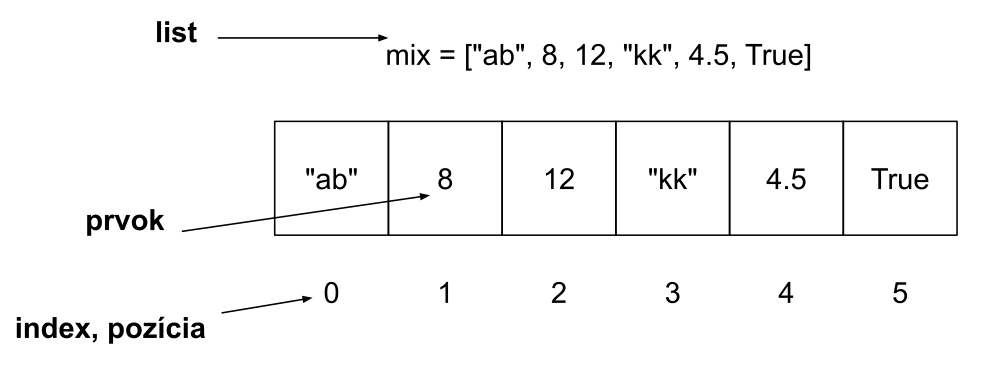
\includegraphics[width=11cm]{list}
\centering
\caption{Ukážka 6-prvkového listu spolu s indexami.}
\end{figure}
Na koniec listov často potrebujeme pridávať hodnotu. Na to slúži \textit{metóda}\footnote{Métoda je funkcia naviazaná na konkrétny \textit{objekt}, pričom objekt v Pythone je všetko (premenné, hodnoty, funckie, ...). Zavolať metódu môžeme ako \texttt{<objekt>.<metoda>()}. Napríklad \texttt{cisla.append(8)}. Môžete si to predstaviť tak, že \texttt{append} je obyčajná funckia, ktorá ako prvý parameter dostane pole \texttt{cisla} a ako druhý parameter $8$.}  \texttt{append} (po slovensky ''pripojiť''). Táto metóda pridá novú hodnotu \textbf{na koniec} listu. Ak chceme pristúpiť k niektorému z prvkov listu, stačí za menom listu pozíciu obaliť do hranatých zátvoriek, teda \texttt{<list>[<pozicia>]}. Napríklad \texttt{cisla[0]}.
\lstlang{python}\begin{lstlisting}
# Program dostane cislo n, pocet cisel, ktore budu nasledovat
# na dalsich riadkoch. Nasledne nacita tieto cisla a vypise ich.
n = int(input())
vstup = []
for i in range(n):
  vstup.append(int(input()))

for i in range(n):
  print(vstup[i])

# Napriklad pre vstup:
3
1
2
3
# Vyda program vystup (tu skratene do jedneho riadku):
1 2 3
\end{lstlisting}

Tento program je možno najkomplexnejší, s ktorým sme sa zatiaľ v tomto návode stretli. Na začiatku načíta číslo $n$, počet čísel, ktoré budú nasledovať na samostatných riadkoch. Následne v cykle od $0$ po $n - 1$ (vrátane) načíta vždy jedno číslo \texttt{int(input())} a pripojí ho do listu $vstup$ pomocou \texttt{append}.

Následne program načítané čísla vypíše. Vo \texttt{for}-cykle od $0$ po $n - 1$ postupne prístupi pomocou premennej $i$ k prvkom poľa na indexoch $0$ až $n - 1$ a vypíše ich.

Posledný cyklus sa dá zapísať trochu jednoduchšie. Samotný \texttt{for} cyklus má totiž hlavičku v tvare \texttt{for <premenna> in <list>:}. Premenná z cyklu teda môže nadobúdať hodnoty z ľubovoľného listu. To znamená, že funkcia \texttt{range}, ktorú sme si uviedli v predošlej kapitole nerobí nič iné ako to, že vytvorí pole.\footnote{Realita je ešte o trošku komplikovanejšia, pretože range je \textit{generátor}, ale priblíženie s listom je dostačujúce.} Skúsme to!
\lstlang{python}\begin{lstlisting}
# Funkciu list, ktora prekonvertuje range na list musime pouzit
# preto, lebo range je "lenivy" a na list sa premeni len ked naozaj musi.
print(list(range(5)))
# Vystup: [0, 1, 2, 3, 4]

print(list(range(0, 10, 2)))
# Vystup: [0, 2, 4, 6, 8]
\end{lstlisting}

Teraz už môžeme \texttt{list} $vstup$ z príkladu, kde sme načítavali $n$ čísel, vypísať trochu jednoduchšie.
\lstlang{python}\begin{lstlisting}
# Do listu "vstup" priradzujeme "natvrdo" hodnoty aby bol tento kod
# spustitelny bez chybovej hlasky.
vstup = [1, 2, 3]

# Premenna "x" postupne nadobudne hodnoty 1, 2, 3.
for x in vstup:
    print(x)
# Vystup (skrateny na jeden riadok):
1 2 3
\end{lstlisting}

Príklady vyššie počítali s tým, že čísla dostaneme rozdelené do riadkov. Čo ak by sme $n$ čísel dostali na jedinom riadku? Funkcia \texttt{input} by ich všetky načítala do jedného reťazca a funkcia \texttt{int} by zlyhala, pretože vie skonvertovať iba \textbf{jedno číslo z reťazca}, nie viacero.
\lstlang{python}\begin{lstlisting}
# Program dostane cislo n, pocet cisel, ktore budu nasledovat
# na dalsom riadku oddelene medzerou.
n = input()
cisla = input()
int(input())
# Chyba!
# Naprilkad pre vstup:
# 3
# 3 4 5
# Dostaneme chybu:
#    ValueError: invalid literal for int() with base 10: '3 4 5'
# To znamena, ze funkcia int() nevie skonvertovat '3 4 5' na jedine cislo.
\end{lstlisting}

Pomôžeme si preto metódou \texttt{split}, ktorá rozseká čísla v reťazci podľa medzier a vráti pole obsahujúce jednotlivé čísla (ako reťazce!).
\lstlang{python}\begin{lstlisting}
# Program dostane cislo n, pocet cisel, ktore budu nasledovat
# na dalsom riadku oddelene medzerou.
n = input()
cisla = input()
# rozsekaneStr, pretoze su to stringy
rozsekaneStr = cisla.split()
print(f'rozsekaneStr: {rozsekaneStr}')

# Z jednotlivych stringov potrebujeme dostat inty
rozsekaneInt = []
for x in rozsekaneStr:
  rozsekaneInt.append(int(x))
  
print(rozsekaneInt)

# Vstup:
3 
3 4 5
# Vystup:
# rozsekaneStr: ['3', '4', '5']
# rozsekaneInt: [3, 4, 5]
\end{lstlisting}

Ukážeme si ešte jeden príklad použitia listu, tentokrát bude obsahovať reťazce. Program má za úlohu vypísať kód mesiaca zo vstupu.
\lstlang{python}\begin{lstlisting}
# Program dostane cislo mesiaca (indexovaneho od 0) a vypise jeho skratku.
mesiace = ["jan", "feb", "mar", "apr", "maj", "jun",
           "jul", "aug", "sep", "okt", "nov", "dec"]
n = int(input())
print(mesiace[n])
\end{lstlisting}

\subsection{Príklady}
\href{https://testovac.ksp.sk/tasks/ls-uvod-zvacsi2/}{Zväčši 2},
\href{https://testovac.ksp.sk/tasks/ls-uvod-sucetmensich/}{Súčet menších},
\href{https://testovac.ksp.sk/tasks/ls-uvod-pocetnajmensich/}{Počet najmenších}

\section{Vnorené cykly}

%TODO (Žaba): tu by sa mi tiež viac páčil postupný prístup, kde najskôr vyriešim jeden riadok a uvidím, že ten sa opakuje tak to zopakujem. Začať niečím ľahším ako násobilkou, kde sa obe veci menia, už len zopakova niekoľkokrát 1 2 3 4 5 je dobrý začiatok imho.
Skúsme vytvoriť program, ktorý načíta číslo $n$ a čísla od $0$ po $n - 1$ vypíše na 3 riadkoch za sebou. To nemôže byť ťažké, nie?
\lstlang{python}\begin{lstlisting}
# Program vypise cisla od 0 po n - 1 ("n" je na vstupe) na 3 riadkoch za sebou.
n = int(input())
for i in range(n):
  print(f' {i}', end='')
print() # novy riadok

for i in range(n):
  print(f' {i}', end='')
print() # novy riadok

for i in range(n):
  print(f' {i}', end='')
print() # novy riadok

# Vstup:
3
# Vystup:
 0 1 2
 0 1 2
 0 1 2
\end{lstlisting}
V tomto programe uvádzame nový konštrukt pre tvorbu reťazca \texttt{f'text \{<premenna>\} text \{<premenna>\}'}. Pomocou uvedenia reťazca so znakom \texttt{f} povolíte tzv. \textit{interpoláciu} premenných pomocou kučeravých zátvoriek. V reťazci sa tak objaví hodnota premennej na mieste, kde bol jej názov v kučeravých zátvorkách. Napríklad \texttt{f'Toto je \{meno\}. Jeho obľúbené zviera je \{zviera\}.'}.

Príklad sme ale uvádzali aj z iného dôvodu. Asi už tušíte, že trikrát skopírovaný \texttt{for}-cyklus nevyzerá najlepšie. Ako by sme teda mohli zopakovať riadky viackrát? No predsa cyklom! V cykle, ktorý sa zopakuje $3$-krát napíšeme cyklus, ktorý vypíše prvky od $0$ po $n - 1$.
\lstlang{python}\begin{lstlisting}
# Program vypise cisla od 0 po n - 1 ("n" je na vstupe) na 3 riadkoch za sebou. Pouziva vnoreny cyklus.
n = int(input())
for i in range(3):
  for j in range(n):
    print(f' {j}', end='')
  print() # novy riadok

# Vstup:
3
# Vystup:
 0 1 2
 0 1 2
 0 1 2
\end{lstlisting}
Dva cykly od seba v označení oddelíme tak, že cyklus opakujúci sa $3$-krát nazveme \textit{vonkajší} a cyklus v ňom nazveme \textit{vnútorný}. Všimnite si, že vnútorný cyklus musí použiť inú premennú ako $i$, pretože inak by došlo ku kolízii mien a vonkajší cyklus by mohol byť ovplyvnený vnútorným. Vo vnútornom cykle sme preto použili názov $j$.
Vždy, keď sa začne vykonávať telo vonkajšieho cyklu, spustí sa znovu vnútorný cyklus vypisujúci čísla od $0$ po $n - 1$.

\subsection{Tabuľka násobilky}
Predstavte si teraz, že chceme vytvoriť malú tabuľku násobilky do $4$. Tabuľka násobilky je jednoduchá tabuľka, ktorá v ľubovoľnej bunke obsahuje vynásobené číslo riadku a stĺpca.
\begin{table}[h]
\begin{center}
\renewcommand\arraystretch{1.3}
\setlength\doublerulesep{0pt}
\begin{tabular}{r||*{4}{2|}}
* & 1 & 2 & 3 & 4 \\
\hline\hline
1 & 1 & 2 & 3 & 4 \\ 
\hline
2 & 2 & 4 & 6 & 8 \\ 
\hline
3 & 3 & 6 & 9 & 12 \\ 
\hline
4 & 4 & 8 & 12 & 16 \\ 
\hline
\end{tabular}
\caption{Tabuľka malej násobilky do 4.}
\end{center}
\end{table}

Teraz napíšeme program, ktorý vypíše telo takejto tabuľky. Ako by sme postupovali, keby sme chceli takúto tabuľku vypísať po riadkoch zľava doprava? V riadku s číslom $1$ sa vystriedajú všetky hodnoty stĺpcov ($1$ až $4$). Potom sa presunieme na ďalší riadok s číslom $2$ a opäť sa vystriedame všetky hodnoty stĺpcov ($1$ až $4$). Takto by sme pokračovali až do posledného riadku.

Všimnite si, že pre každý riadok prejdeme vždy všetky stĺpce. Môžeme si to predstaviť ako cyklus cez riadky od $1$ do $4$, v ktorom je navyše \textit{vnorený} cyklus cez stĺpce od $1$ do $4$.
\lstlang{python}\begin{lstlisting}
# Vypis tabulky nasobilky velkosti 5x5.
for i in range(1, 5):
  for j in range(1, 5):
    # Medzeru medzi cislami nevypisujeme pred prvym cislom v riadku
    if j > 1:
       print(' ', end='')
    print(i * j, end='')
  print() # novy riadok
\end{lstlisting}

Za zmienku ešte stojí spomenúť chovanie \texttt{break} a \texttt{continue} vo vnorených cykloch. Oba príkazy sa viažu na \textit{najbližší uzatvárajúci} cyklus. To napríklad znamená, že z vnoreného cyklu sa nedá vyskočiť "úplne" (mimo cyklov), ale iba do vonkajšieho cyklu.
\lstlang{python}\begin{lstlisting}
# Program vypisuje dvojice cisel od 0 po 8 v poradi od najmensich
# dvojic az pokial prve cislo nie je delitelne 3 a zaroven druhe cislo
# nie je delitelne 2.
for i in range(8):
  for j in range(8):
    # Chyba! Z vonkajsieho cyklu nevyskocime!
    if i % 3 == 0 and j % 2 == 0:
      break
    # Vypise i a j oddelene medzerou, ekv. s f'{i} {j}'.
    print(i, j)

# Vystup:
0 0
0 1
...
0 7
1 0
...
3 1
# 3 2 sa nevypise, ale program pokracuje (chyba!)
4 0
4 1
...
\end{lstlisting}

V prípade, že by sme v príklade vyššie použili \texttt{continue} namiesto \texttt{break} by ďalšia vypísana dvojica bola po vynechanej ($3$ $2$) bola
($3$ $3$), pretože z vnútorného cyklu by sme nevyskočili úplne, ale iba preskočili výpis.

\section{List listov}
Keď už vieme vnárať cykly, asi vás neprekvapí, že vnárať sa dajú aj listy :)
Napríklad tu je list listov, ktorý obsahuje informácie o domácich zvieratách jedného z vedúcich.
\lstlang{python}\begin{lstlisting}
zvierata = [
  ["Bax", "pes", "ciernobiely"],
  ["Kralovna", "macka", "biela"],
  ["Fero", "kocur", "hnedobiely"]
]
\end{lstlisting}
Všimnite si, že list \texttt{zvierata} obsahuje $3$ ďalšie listy. Každý z týchto $3$ listov popisuje jedno zviera. List konkrétneho zvieraťa obsahuje jeho meno, typ a farbu.

Vnorené listy indexujeme rovnako ako jednorozmerné. Keď teda zaindexujeme do listu \texttt{zvierata}, dostaneme list.
\lstlang{python}\begin{lstlisting}
# zvierata = ...z predzchadzajuceho prikladu...

print(zvierata[1])
# Vystup (list): ["Kralovna", "macka", "biela"]
\end{lstlisting}
Tento list môžeme opäť indexovať.
\lstlang{python}\begin{lstlisting}
# zvierata = ...z predzchadzajuceho prikladu...

# Farba prveho (nulteho) zvierata
print(zvierata[0][2])
# Vystup: "ciernobiely"
\end{lstlisting}
Skúsme teraz napísať program, ktorý vypíše mená všetkých zvierat.
\lstlang{python}\begin{lstlisting}
# zvierata = ...z predzchadzajuceho prikladu...

for zviera in zvierata:
  print(zviera[0])

# Vystup (skrateny na jeden riadok):
Bax Kralovna Fero
\end{lstlisting}
Vo for cykle prejdeme cez vsetky \texttt{zvierata}. Premenná \texttt{zviera} bude preto postupne obsahovať polia \texttt{["Bax", "pes", "ciernobiely"]} až
\texttt{["Fero", "kocur", "hnedobiely"]}. Z týchto polí potom vypisujeme $0$-tú hodnotu, čo je meno.

Ako načítať \textit{dvojrozmerné pole}\footnote{Dvojrozmerné pole môže znieť odstrašujúco, ale s tým, čo už vieme, je vysvetlenie hračka. Je to jednoducho list listov. Pole je list a dvojrozmerné sa volá preto, lebo je to v podstate tabuľka, v ktorej môžeme chodiť po riadkoch aj stĺpcoch.} (tabuľku čísel)? Pomocou vnorených cyklov.
\lstlang{python}\begin{lstlisting}
# Program dostane cisla m a n na jednom riadku, pocet riadkov a pocet stlpcov tabulky.
# Nasledne dostane jednotlive hodnoty tabulky.

rozmery = input().split()
# Trik: skratka za
# m = int(rozmery[0])
# n = int(rozmery[1])
m, n = int(rozmery[0]), int(rozmery[1])

tabulka = []
for i in range(m):
  riadokStr = input().split()
  riadokInt = []
  for x in riadokStr:
    riadokInt.append(int(x))
  tabulka.append(riadokInt)

print(tabulka)

# Vstup:
3 4
1 2 3 4
5 6 7 8
9 10 11 12
# Vystup:
[
 [1, 2, 3, 4],
 [5, 6, 7, 8],
 [9, 10, 11, 12]
]
\end{lstlisting}

\subsection{Príklady}
\href{https://testovac.ksp.sk/tasks/ls-uvod-rozdiel/}{Rozdiel},
\href{https://testovac.ksp.sk/tasks/ls-uvod-suctovapyramida/}{Súčtová pyramída},
\href{https://testovac.ksp.sk/tasks/ls-uvod-vymena/}{Výmena},
\href{https://testovac.ksp.sk/tasks/ls-uvod-otocenie/}{Otočenie}

\section{Funkcie}

Predstavte si, že vo svojom programe potrebujete často urobiť to isté. Napríklad potrebujete na viacerých miestach zistiť, či je číslo párne a odpoveď vypísať. Samozrejme môžete použiť \texttt{if} a \texttt{print} na všetkých miestach kde danú vec potrebujete pričom by to vyzeralo nejak takto:

\lstlang{python}\begin{lstlisting}
if x%2 == 0:
    print("Parne cislo.")
else:
    print("Neparne cislo.")
#   
#
#
if a%2 == 0:
    print("Parne cislo.")
else:
    print("Neparne cislo.")
#
#
# a tak dalej
\end{lstlisting}

Toto síce docieli to čo chceme avšak za následok to bude mať aj dlhší, neprehľadnejší kód s viac miestami kde sa môžeme pomýliť. Nezúfajte, zachránia nás funkcie. Horný program môžeme ekvivalentne zapísať aj krajšie:

\lstlang{python}\begin{lstlisting}
def vypisParitu(cislo)
    if cislo%2 == 0:
        print("Parne cislo.")
    else:
        print("Neparne cislo.")
#   
#
vypisParitu(x)
#
#
vypisParitu(a)
#
# a tak dalej
\end{lstlisting}

Ak si predchádzajúce dva príklady porovnáte, malo by vám byť intuitívne jasné, čo funkcie robia. S funkciami sme sa už stretli kedže \texttt{print} je príklad funkcie. Čo je teda funkcia? Je to viac príkazov pospájaných do jedného celku, tvoriac akýsi superpríkaz vykonávajúci nejakú vec. Pamätajte, funkcia môže mať aj niekoľko desiatok riadkov pokiaľ toho robí viac alebo je zložitejšia. Prvá vec, ktorú máme možnosť vidieť v príklade vyššie je, že funkcia má parameter/parametre. Parametre sa uvádzajú do zátvoriek za funkciou a ide o cestu, ako funkcii odovzdať nejakú informáciu. V prípade vyššie má funkcia \textit{vypisParitu} jeden parameter s názvom cislo. Tento parameter má táto funkcia preto, že jej nejak chceme odovzdať číslo, ktoré potrebuje k rozhodnutiu sa, čo vypísať. Keď chceme funkciu použiť, hovoríme, že ju voláme a teda v programe vidíme dve volania funkcie \textit{vypisParitu}. Pri volaní funkcii odovzdáme naše číslo ako parameter.

Okrem toho, že si funkcie berú parametre, vedia niečo aj vracať. Funkcia vyššie nič nevracia. Ak by sme ale chceli vidieť príklad toho, ako môže funkcia niečo vracať, môže to vyzerať takto.

\lstlang{python}\begin{lstlisting}
def scitaj(a, b)
    return a+b
# pouzitie:
x, y = 10, 20
vysledok1 = scitaj(x, y)
vysledok2 = scitaj(x, 77)
vysledok3 = scitaj(5, 11)
\end{lstlisting}

Vyššie vidíme veľmi jednoduchú funkciu, ktorá iba sčíta svoje parametre a vráti ich pomocou kľúčového slova \texttt{return} a potom 3 rôzne korektné použitia tejto funkcie.

Jedna z dôležitých vecí je, ako funguje premenná potom, čo sa stane parametrom. Pokiaľ napíšeme jednoduchý program.

\lstlang{python}\begin{lstlisting}
def zmen(x):
    x = 30
a = 10
print(a)
zmen(a)
print(a)
\end{lstlisting}

Po jeho spustení zistíme, že sa hodnota premennej $a$ po zmene vo funkcii \texttt{zmen} nezmenila. Je to spôsobené tým, že do funkcie nebola poslaná priamo premenná $a$ ale len jej kópia, ktorá sa po konci vykonávania funkcie zahodí. Veci sa ale trocha skomplikujú keď spustíme nasledujúci program.

\lstlang{python}\begin{lstlisting}
def zmen(x):
    x[0] = 30
a = [1, 2, 3]
print(a)
zmen(a)
print(a)
\end{lstlisting}

Čakali by sme, že sa $a$ nezmení avšak tentokrát je $a$ \texttt{list}. Prečo sa v tomto prípade zmenila hodnota $a$? Je to z dôvodu, že do funkcie bola v tomto prípade poslaná nie kópia listu ale priamo list $a$. Je trochu nelogické, prečo sa python správa rôzne pri rôznych typoch. Je to napríklad z dôvôdu, že listy sú zväčša pomerne veľké, zaberajú viac miesta a teda aj ich kopírovanie je pomalé a Python sa mu snaží vyhnúť. Je dôležité si na toto správanie dávať pozor a keď je to dôležité, vyskúšať ako sa Python správa pre konkrétny typ.

\subsection{Príklady}
\href{https://testovac.ksp.sk/tasks/ls-uvod-tlacitka/}{Tlačítka}

\section{Záver}

Super! Ak si to dotiahol až sem a popri tom urobil všetky úlohy tak máš solídne základy v jazyku Python. Veríme, že tvoja programátorská cesta tu nekončí. Čaká ťa totiž veľa zaujimávych príležitostí, kde svoju znalosť jazyka Python môžeš ďalej prehĺbiť. Ďakujeme, že si čítal náš tutoriál a najväčším poďakovaním bude ak nám povieš, čo v ňom môžeme zlepšiť aby sa ďalším čitateľom čítal jednoduchšie. Kontaktovať nás môžeš buď na Discorde pod nickom sobkulir a Aj0SK alebo na adresách andrejkorman@gmail.com a r.sobkuliak@gmail.com. Tiež nás kontaktuj ak nevieš kam s tvojimi znalosťami ďalej :)

% \nadpis{Slovník}
% argument
% parameter
% funkcia?
% iteracia
% riadiaca premenna cyklu
% odsadený

% \kapitola{Aux veci}
% Teraz si ukážeme jeden často používaný trik. Listy sa dajú násobiť \texttt{<pocet> * <list>}. Tento výraz vytvorí nový \texttt{list}, v ktorom sa \texttt{<list>} opakuje za sebou \texttt{pocet}-krát.
% \lstlang{python}\begin{lstlisting}
% # "Nasobenie listu" - prikaz vytvori list obsahujuci 4-krat hodnotu 10.
% B = 4 * [10]
% [10, 10, 10, 10]
% \end{lstlisting}

% Nižšie je príklad 
% A takisto, keďže aj list je len typ premennej, viem robiť listy viacrozmerné -- listy listov.
% Tieto listy, si môžeme predstaviť ako tabuľky. Jedno číslo použijeme na nájdenie
% riadku, druhé na nájdenie stĺpca.

% \lstlang{python}\begin{lstlisting}
% K = [ [None] * 5 for i in range(10) ] # vytvori list velkosti 10 * 5
% K[4][5] = 18 # do 5. riadku a 6. stlpca ulozi 15

% # POZOR! takto vytvoreny dvojrozmerny list sa nebude spravat ako chceme
% ZLE = [[1] * 3] * 5    
% print(ZLE)   # vypise[[1, 1, 1], [1, 1, 1], [1, 1, 1], [1, 1, 1], [1, 1, 1]]
% ZLE[0][1] = 2    # chceme zmenit prvok v 1. riadku a 2. stlpci
% print(ZLE)    # vypise [[1, 2, 1], [1, 2, 1], [1, 2, 1], [1, 2, 1], [1, 2, 1]]
% \end{lstlisting}

\end{document}